\documentclass[UTF8]{ctexart}
\usepackage{color} 
\usepackage{bm}
\usepackage{algorithm}
\usepackage{algpseudocode}
\usepackage{multirow}
\usepackage{indentfirst}
\usepackage{subfigure}
\usepackage{epsfig}
\usepackage{epstopdf}
\usepackage{xspace}
\usepackage{amsmath,amssymb}
\DeclareMathOperator*{\argmax}{arg\,max}
\DeclareMathOperator*{\argmin}{arg\,min}

\floatname{algorithm}{算法}
\renewcommand{\algorithmicrequire}{\textbf{输入:}}
\renewcommand{\algorithmicensure}{\textbf{输出:}}
\usepackage{geometry}

\geometry{a4paper,scale=0.8}

\usepackage{subeqnarray}
\begin{document}

\title{基于期望最大化EM算法估计混合高斯模型GMM参数}
\author{作者}
%\date{January 25, 2015}
\maketitle

\section{理论}

EM算法也称作期望最大化(Expectation-Maximization,简称EM)算法,它是一种迭代算法,
用于含有隐变量的概率模型\textbf{参数}的极大似然估计或极大后验概率估计。

\subsection{极大似然估计}
\label{subsection-1}

极大似然估计(Maximum likelihood estimation,简称MLE)就是利用已知的样本结果(数据)信息,
反推最\textbf{具有可能(最大概率)}导致这些样本结果(数据)出现的模型参数值。

考虑图\ref{MLE},红色叉号表示数据点,这组数据上方有三个高斯分布。
现在假设这组数据全部来自于同一个分布,那最有可能是哪一个分布呢?
我们都知道,高斯分布的参数为$\theta=\{\mu, \sigma\}$,那么问题其实可以表述为:图\ref{MLE} 中三个分布
对应的三组参数里,哪组参数能够更好的解释数据?即哪组参数让这些数据样本出现的可能性最大?

\begin{figure}[!h]
  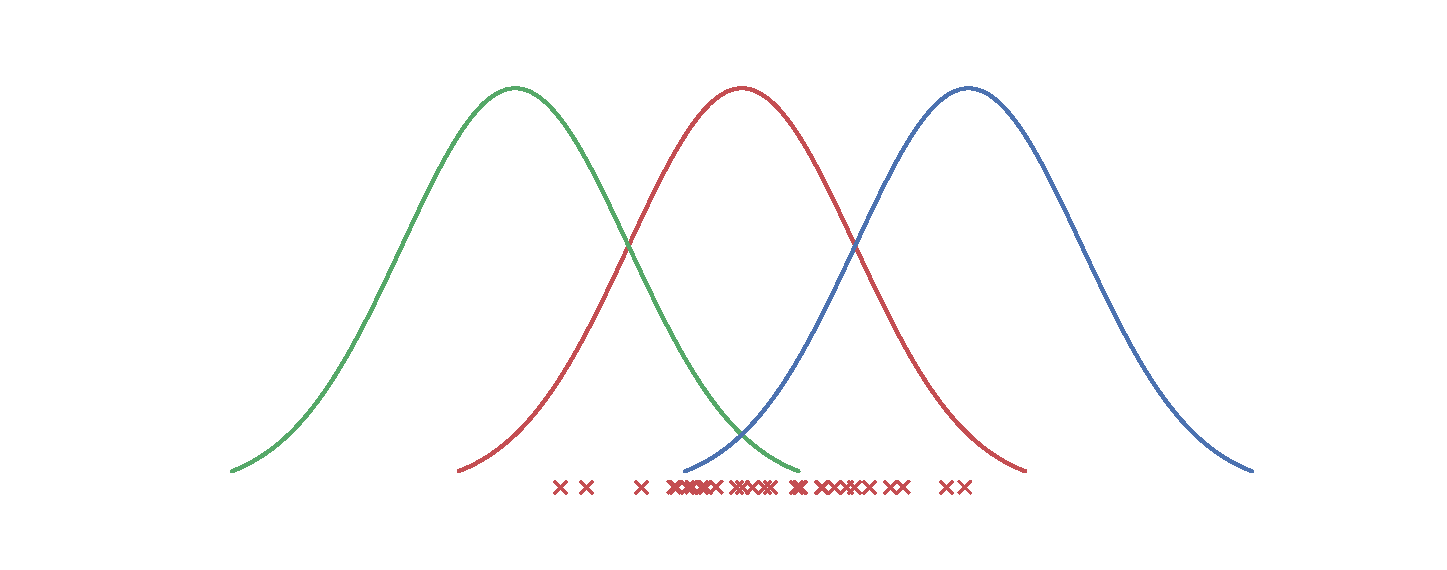
\includegraphics[width=0.5\textwidth]{./figures/MLE.pdf}
  \centering
  \caption{MLE估计高斯分布参数}
  \label{MLE}
\end{figure}

假设数据点表述为$\mathcal{X}=\{x_1, x_2, \cdots, x_n\}$,且每个数据点之间都满足独立同分布条件,
其概率密度函数为$P(X=x|\theta)$,那么所有数据出现的概率就是
\begin{equation}\label{Likelihood}
  \begin{split}
    P(\mathcal{X}|\theta) = \prod_{i=1}^{n}P(x_i|\theta).
  \end{split}
\end{equation}
可以看到公式中数据$\mathcal{X}$是已知的,所以$P(\mathcal{X}|\theta)$是一个关于$\theta$的函数,通常被称作\textbf{似然函数}。

接下来就要寻找能够更好地解释这组数据的参数$\theta$,即使得函数$P(\mathcal{X}|\theta)$的值最大的$\theta$,
写作
\begin{equation}\label{}
  \hat\theta = \argmax_{\theta} \prod_{i=1}^{n}P(x_i|\theta).
\end{equation}
要最大化一个函数的值,我们首先想到的一定是一阶导数为零。但是观察公式 (\ref{Likelihood}),
对于连乘的函数求导并不是一件容易的事情,于是考虑取对数简化运算。

这里有两点考虑:一方面,对数函数能够保持原函数的增减性,所以取对数前后函数的极值点保持一致;
另一方面,对数函数能够变乘法为加法,大大降低了运算难度,也提高了数值的可识别性,
比如概率累乘会出现数值非常小的情况(像1e-30这样的数值),很容易超出计算机的精度产生溢出错误,
而取对数之后,计算机就很容易识别了(对1e-30取以10为底的对数得到-30)。
于是\textbf{对数似然函数}便产生了,如公式 (\ref{LogLikelihood}),
\begin{equation}\label{LogLikelihood}
  \begin{split}
    \mathcal{L}(\theta|\mathcal{X}) &= \mathrm{log}P(\mathcal{X}|\theta)\\
    &= \mathrm{log}\prod_{i=1}^{n}P(x_i|\theta)\\
    &= \sum_{i=1}^{n}\mathrm{log}P(x_i|\theta).
  \end{split}
\end{equation}
注意这里的对数似然函数写成$\mathcal{L}(\theta|\mathcal{X})$而不是$\mathcal{L}(\theta)$,
是因为待估计量(参数)$\theta$是随着观测数据$\mathcal{X}$的变化而变化的。因此优化目标变为:
\begin{equation}\label{}
  \hat\theta = \argmax_{\theta} \sum_{i=1}^{n}\mathrm{log}P(x_i|\theta).
\end{equation}
接下来便是对多维参数求偏导(若是一维参数则直接求导),然后令一阶导数为零,最后一一解出参数的估计值即可。

这里我们以高斯分布为例,进行参数的极大似然估计。

首先高斯分布的概率密度函数为
\begin{equation}
  p(x)= \frac{1}{\sqrt{2 \pi} \sigma}\mathrm{exp}\left(-\frac{(x-\mu)^2}{2\sigma^2}\right),
\end{equation}
假设数据为$X = (x_1,x_2, \cdots,x_n)^T, \quad x_i  \overset{\text{iid}}{\sim} \mathcal{N}(\mu,\sigma^2)$,
可以得到对数似然函数
\begin{equation}
  \begin{split}
    \mathcal{L}(\mu,\sigma|X) &= \sum_{i=1}^{n}\mathrm{log}P(x_i|\mu, \sigma)\\
    &= \sum_{i=1}^{n}{\mathrm{log}\frac{1}{\sqrt{2 \pi} \sigma}\mathrm{exp}\left(-\frac{(x-\mu)^2}{2\sigma^2}\right)}\\
    &= \sum_{i=1}^{n}{\mathrm{log}\frac{1}{\sqrt{2\pi}}+\mathrm{log}\frac{1}{\sigma}-\frac{(x_i-\mu)^2}{2\sigma^2}}.
  \end{split}
\end{equation}
然后用$\mathcal{L}(\mu,\sigma|X)$分别对参数$\mu$和$\sigma$求偏导并令其为零,因为比较容易,
所以这里省略化简过程,最后可以得到参数的估计值:
\begin{equation}
  \begin{split}
    &\hat\mu_{MLE} = \frac{1}{n}\sum_{i=1}^{n}x_i\\
    &\hat\sigma_{MLE}^2= \frac{1}{n}\sum_{i=1}^{n}(x_i-\mu_{MLE})^2.
  \end{split}
\end{equation}
不难发现,用极大似然估计的高斯分布$\hat\mu$为所有样本数据点的均值,$\hat\sigma^2$为所有样本数据点方差。

最后,简单总结一下极大似然估计参数的过程:
\begin{itemize}
  \item[i.] 根据概率密度函数写出似然函数
  \item[ii.] 对似然函数取对数,整理表达式
  \item[iii.] 对表达式求一阶导,令导数为零,得到似然方程
  \item[iv.] 解似然方程,得到参数的估计值
\end{itemize}

\subsection{隐变量}
\label{subsection-2}

在EM算法的学习过程中,经常会看到一个词:\textbf{隐变量}(latent variable),
它是相对于\textbf{观测变量}(obeservable variable)而言的,观测变量一般就指的是数据本身,
那么隐变量到底是什么呢?其实就是未观测到的但是影响观测数据的变量。

下面我们举例进行解释。刚刚在极大似然估计的过程中存在一个假设:所有的数据点来自于同一个分布。
当然这个假设在直观上也是符合认知的,因为图\ref{MLE} 中的那组数据看起来确实像是从同一个高斯分布中抽取出来的。

但是并不是所有问题都符合这种假设,更多的是图\ref{latent variable-1} 中的数据分布,如果我们依旧用单个高斯分布去拟合,
根据章节\ref{subsection-1} 中讨论过的极大似然估计的结果,$\hat\mu$($\mu$的估计值)为样本均值,
$\hat\sigma^2$($\sigma^2$的估计值)为样本方差,因此就会出现图\ref{latent variable-1} 中的情况。
显然,这不是我们想要的。

\begin{figure}[!h]
  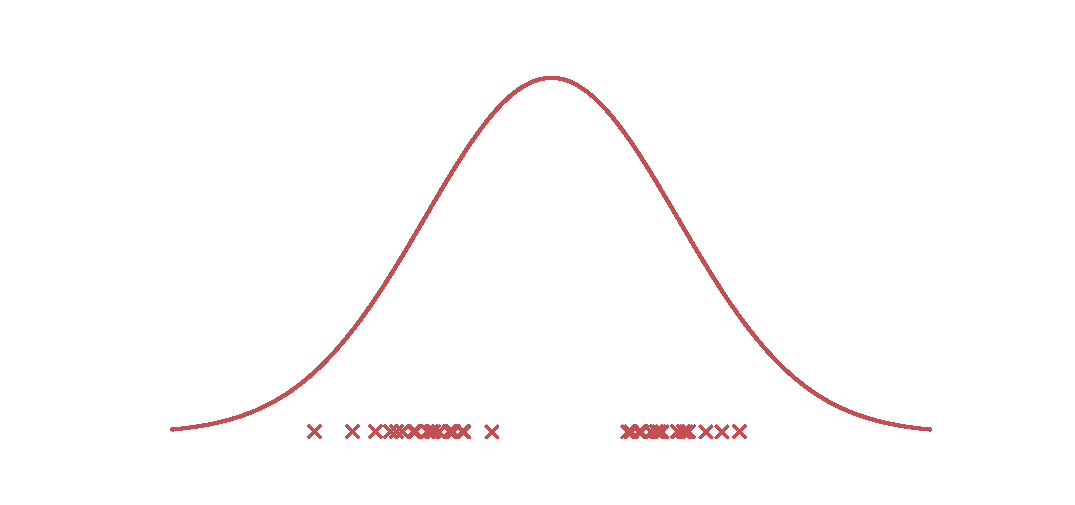
\includegraphics[width=0.5\textwidth]{./figures/LV-1.pdf}
  \centering
  \caption{单高斯拟合含有隐变量的数据}
  \label{latent variable-1}
\end{figure}

很容易想到:我们可以用两个高斯去拟合。这其实就是混合高斯模型的雏形,
其模型思想很简单,如图\ref{latent variable-2} 所示,
当给出的样本是绿色的点时,就用绿色的高斯分布去拟合,
当给出的样本是红色的点时,就用红色的高斯分布去拟合。

\begin{figure}[!h]
  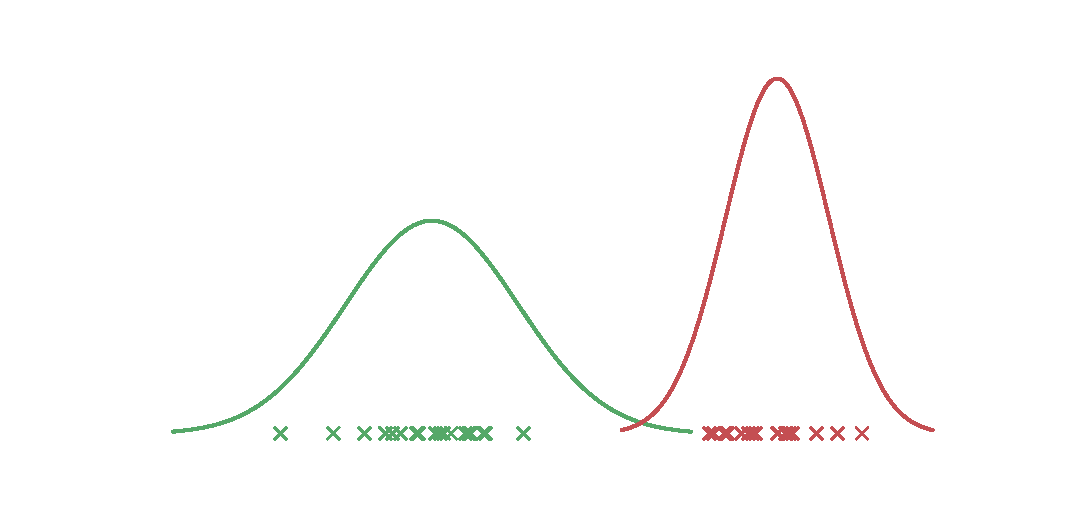
\includegraphics[width=0.5\textwidth]{./figures/LV-2.pdf}
  \centering
  \caption{混合高斯拟合含有隐变量的数据}
  \label{latent variable-2}
\end{figure}

于是,在这个模型中,每一个样本点的解释就分为两步:
第一,这个样本来自于哪个高斯分布,第二,这个高斯分布的参数是什么。
此时\textbf{隐变量}就出现了,它存在于第一步中,用于决定样本来自于哪个高斯分布。
为了让模型更具一般性,假设有$K$个高斯分布,用$z_k={1, 2, \cdots, K}$来表示样本来自于哪个高斯分布,
参数$\theta=\{\mu_1, \cdots, \mu_K; \sigma_1, \cdots, \sigma_K\}$表示每个高斯分布的参数,
那么模型就可以写作:
\begin{equation}
  \begin{split}
    p(x|\theta) &= \sum_{i=1}^{K}p(z_k) \mathcal{N}(\mu_k, \sigma_k)\\
    & \quad\quad \mathrm{s.t.} \quad \sum_{i=1}^{K}p(z_k) = 1,
  \end{split}
\end{equation}
即任意一个样本产生的概率既与决定该样本属于哪个分布的隐变量(此处为$z_k$)有关,
也与产生该样本的分布(此处$\mathcal{N}(\mu_k, \sigma_k)$)有关。

如果将观测数据表示为$X=(x_1, x_2, \cdots, x_n)$,则观测数据的对数似然函数为:
\begin{equation}\label{LogSum}
  \begin{split}
    \mathcal{L}(\theta|X) &= \sum_{i=1}^{n}\mathrm{log}p(x|\theta)\\
    &= \sum_{i=1}^{n}\mathrm{log}\sum_{k=1}^{K}p(z_k) \mathcal{N}(\mu_k, \sigma_k).
  \end{split}
\end{equation}
考虑求模型参数$\theta$的极大似然估计,即
\begin{equation}\label{MaxLLH}
  \hat\theta = \argmax_{\theta}\mathcal{L}(\theta|X).
\end{equation}
按照极大似然估计的步骤,我们应该给$\mathcal{L}(\theta|X)$求偏导并令其为零,然后求解方程得到参数的估计值。

但是从公式(\ref{LogSum}) 可以看到,由于\textbf{隐变量}的引入,
$\mathcal{L}(\theta|X)$的表达实里存在求和之后取对数的情况,
这时想要求导并得到解析解几乎不可能,因此只有通过迭代的方法求解,
而EM算法就是可以用于求解这个问题的一种迭代算法。

\subsection{EM算法}

对于一个迭代算法而言,必须有一个迭代变量,同时也要建立起一个迭代关系,如公式(\ref{IterativeFunction}),
从而让计算机发挥运算速度快、适合做重复运算的优势来进行求解。
\begin{equation}\label{IterativeFunction}
  \theta^{(g+1)} = f \left (\theta^{(g)} \right).
\end{equation}

既然EM算法是一种迭代算法,那么它的迭代变量和迭代关系分别是什么呢?
通常会看到教科书或者网课上给出如公式(\ref{IF4EM}) 所示的迭代关系,
其中,$X$代表所有数据样本,$Z$ 代表隐变量,$\theta$是模型参数,其右上角的角标代表迭代轮数。
\begin{equation}\label{IF4EM}
  \textcolor[rgb]{0.0,0.0,0.8}{\theta^{(g+1)} = \argmax_{\theta} \int_{Z}\mathrm{log}P (X, Z | \theta) P \left(Z|X, \theta^{(g)} \right)dZ}.
\end{equation}
但是为什么是这样的迭代关系呢?我们一步步来分析。

首先,假设迭代关系是对数似然函数,既然我们想要最大化它的值,那么就需要保证每一步迭代的结果都比上一次更好,
即证明
\begin{equation}
  \mathcal{L} \left(\theta^{(g+1)}|X \right) \ge \mathcal{L} \left(\theta^{(g)}|X \right),
\end{equation}
也可以将其展开,
\begin{equation}\label{EMCondition}
  \textcolor[rgb]{0.0,0.0,0.8}{\mathrm{log}P \left(X|\theta^{(g+1)} \right) \ge \mathrm{log} P \left(X|\theta^{(g)}\right)}.
\end{equation}

可以看到,目前为止隐变量还没有出现,下面来看对数似然函数本身,我们结合贝叶斯公式引入隐变量$Z$,
试图简化计算,
\begin{equation}\label{BeforeE}
  \begin{split}
    \mathrm{log}P(X|\theta) &= \mathrm{log} \left\{ \frac{P(X,Z|\theta)}{P(Z|X, \theta)}\right\}\\
    &= \mathrm{log}P(X,Z|\theta) - \mathrm{log}P(Z|X,\theta),
  \end{split}
\end{equation}
然后对其两边依照概率$P(Z|X,\theta^{(g)})$求期望,
\begin{equation}
  \mathbb{E}_{P(Z|X,\theta^{(g)})}\left[\mathrm{log}P(X|\theta)\right] = \mathbb{E}_{P(Z|X,\theta^{(g)})}\left[\mathrm{log}P(X,Z|\theta)\right] - \mathbb{E}_{P(Z|X,\theta^{(g)})}\left[\mathrm{log}P(Z|X,\theta)\right],
\end{equation}
将其写为积分的形式,由于$\mathrm{log}P(X|\theta)$中不含积分变量$Z$,所以先将其提到积分运算之外,
\begin{equation}\label{IntegerSimplify}
  \begin{split}
    \int_{Z}\mathrm{log}P(X|\theta)P\left(Z|X,\theta^{(g)}\right)dZ &= \int_{Z}\mathrm{log}P(X,Z|\theta)P\left(Z|X,\theta^{(g)}\right)dZ - \int_{Z}\mathrm{log}P(Z|X,\theta)P\left(Z|X,\theta^{(g)}\right)dZ\\
    \mathrm{log}P(X|\theta)\int_{Z}P\left(Z|X,\theta^{(g)}\right)dZ &= \int_{Z}\mathrm{log}P(X,Z|\theta)P\left(Z|X,\theta^{(g)}\right)dZ - \int_{Z}\mathrm{log}P(Z|X,\theta)P\left(Z|X,\theta^{(g)}\right)dZ,
  \end{split}
\end{equation}
因为变量空间中所有事件的概率和为1,即$\int_{Z}P(Z|X,\theta^{(g)})dZ = 1$,因此可以将上式化简为
\begin{equation}\label{QH}
  \textcolor[rgb]{0.0,0.0,0.8}{\mathrm{log}P(X|\theta) = \underbrace{\int_{Z}\mathrm{log}P(X,Z|\theta)P\left(Z|X,\theta^{(g)}\right)dZ}_{Q\left(\theta,\theta^{(g)}\right)} - \underbrace{\int_{Z}\mathrm{log}P(Z|X,\theta)P\left(Z|X,\theta^{(g)}\right)dZ}_{H\left(\theta, \theta^{(g)}\right)}}.
\end{equation}

至此,我们有一个问题还没有考虑:为什么要依照概率$P(Z|X,\theta^{(g)})$求期望呢?
$P(Z|X,\theta^{(g)})$代表了给定观测数据$X$和第$g$轮参数估计$\theta^{(g)}$下隐变量数据$Z$的
条件概率分布,由于$Z$是未观测数据,是用于简化计算的辅助变量,所以必须保证它不能影响结果,
也就是说在求第$g+1$轮的参数估计$\theta^{(g+1)}$时,必须保证在给定数据$X$的情况下,
$\theta$是唯一影响对数似然函数取值的因素,这就要求剔除$Z$的影响,
因而对公式(\ref{BeforeE}) 依照概率$P(Z|X,\theta^{(g)})$求期望从而将$Z$消掉。

回到证明EM算法的收敛性上来,即证明公式(\ref{EMCondition}) 成立,结合公式(\ref{QH}) 可将问题转化为
证明下式成立:
\begin{equation}\label{EMFinalCondtion}
  Q \left(\theta^{(g+1)},\theta^{(g)}\right) - H\left(\theta^{(g+1)}, \theta^{(g)}\right) \ge Q\left(\theta^{(g)},\theta^{(g)}\right) - H\left(\theta^{(g)},\theta^{(g)}\right).
\end{equation}

不难发现,公式(\ref{QH}) 中的$Q\left(\theta,\theta^{(g)}\right)$其实就是EM算法迭代函数中最大化的对象,
结合它将公式(\ref{IF4EM}) 改写一下可以得到:
\begin{equation}\label{QFunction}
  \forall \theta, Q \left(\theta^{(g+1)},\theta^{(g)}\right) \ge Q\left(\theta,\theta^{(g)}\right).
\end{equation}
也就是说,左边式子是个值,右边式子是个函数,而且不论右边式子中的变量$\theta$取任何值,都不会大于左边式子的值,
因而左边式子的值是右边函数的最大值,所以当$\theta = \theta^{(g)}$时,上式依然成立,即
\begin{equation}\label{Qresult}
  Q \left(\theta^{(g+1)},\theta^{(g)}\right) \ge Q\left(\theta^{(g)},\theta^{(g)}\right).
\end{equation}

接下来证明$H$项,既然$Q$项已经满足公式(\ref{Qresult}) 了,那么如果$H$项能满足
\begin{equation}\label{Hresult}
  H \left(\theta^{(g+1)},\theta^{(g)}\right) \le H\left(\theta^{(g)},\theta^{(g)}\right).
\end{equation}
我们就可以完成公式(\ref{EMFinalCondtion})证明了。
要证明上式成立,我们也可以构造类似公式(\ref{QFunction}) 的不等式,即
\begin{equation}\label{HFunction}
  \forall \theta, H\left(\theta,\theta^{(g)}\right) \le H \left(\theta^{(g)},\theta^{(g)}\right).
\end{equation}
如果这个式子成立,那么就可以同样的令$\theta = \theta^{(g+1)}$从而证明公式(\ref{Hresult}) 成立。
要证这个式子成立,需要参考公式(\ref{QH})和Jensen不等式,有
\begin{equation}\label{HProve}
  \begin{split}
    & H \left(\theta,\theta^{(g)}\right) - H \left(\theta^{(g)},\theta^{(g)}\right)\\
    =& \int_{Z}\mathrm{log}P(Z|X,\theta)P\left(Z|X,\theta^{(g)}\right)dZ - \int_{Z}\mathrm{log}P(Z|X,\theta^{(g)})P\left(Z|X,\theta^{(g)}\right)dZ\\
    =& \int_{Z}\mathrm{log}\frac{P(Z|X,\theta)}{P\left(Z|X,\theta^{(g)}\right)}P\left(Z|X,\theta^{(g)}\right)dZ\\
    \le& \mathrm{log}\int_{Z}\frac{P(Z|X,\theta)}{P\left(Z|X,\theta^{(g)}\right)}P\left(Z|X,\theta^{(g)}\right)dZ\\
    =& \mathrm{log}\int_{Z}P(Z|X,\theta)dZ\\
    =& \mathrm{log}1\\
    =& 0
  \end{split}
\end{equation}
因而公式(\ref{HFunction}) 是成立的,所以公式(\ref{EMFinalCondtion}) 得证。
综上所述,EM算法是会随着迭代的进行一步步收敛到极值的。

在公式(\ref{HProve}) 的证明中,出现不等式的那一步利用了所谓的Jensen不等式,
简单来讲,Jensen不等式描述了:在凸函数中(这里指下凸函数),
函数的期望不小于期望的函数,或者说
在凹函数中,函数的期望不大于期望的函数。

其实它很容易理解,如图\ref{FigJensen} 所示,
可以看到,对于点$x1$和$x2$,
函数的期望为$p1*f(x1)+p2*f(x2)$,期望的函数为$f(p1*x1+p2*x2)$,
显然,假设约束$p1+p2=1, p1>0, p2>0$一直满足,那么无论$p1$和$p2$如何变化,
$p1*f(x1)+p2*f(x2) \le f(p1*x1+p2*x2)$总是成立,即函数的期望总是不大于期望的函数。

\begin{figure}[!h]
  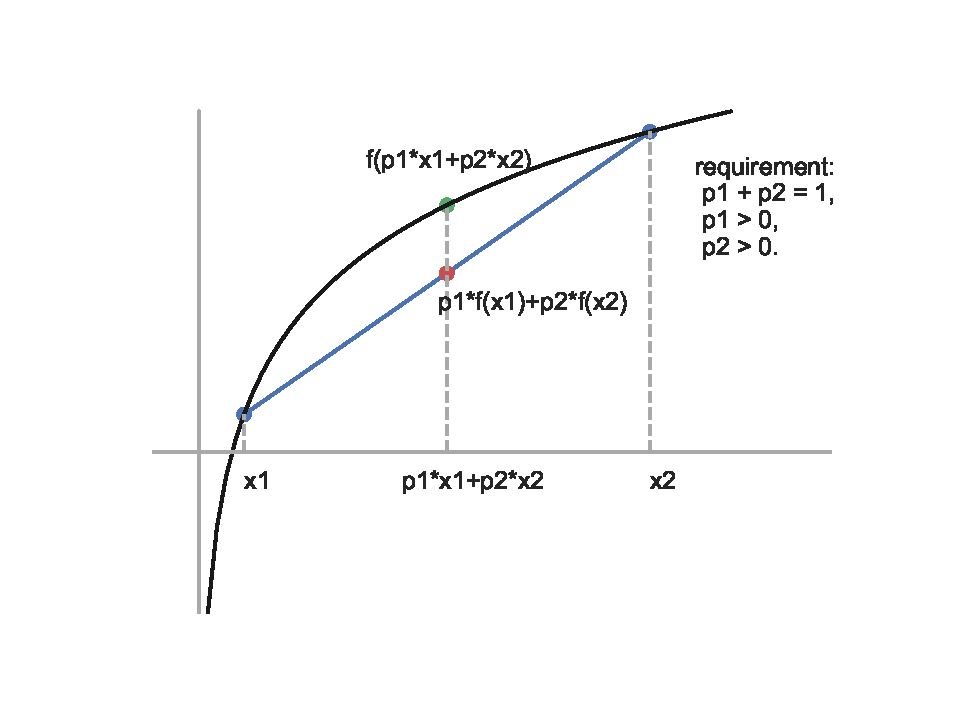
\includegraphics[width=0.5\textwidth]{./figures/Jensen.pdf}
  \centering
  \caption{Jensen不等式图示}
  \label{FigJensen}
\end{figure}

结合公式(\ref{HProve}) 来说,这里的函数指的是$\mathrm{log(x)}$,
而对于连续的变量通常使用积分来替代期望,所以下式很容易成立,
\begin{equation}\label{JensenInHP}
  \int_{Z}\mathrm{log}\frac{P(Z|X,\theta)}{P\left(Z|X,\theta^{(g)}\right)}P\left(Z|X,\theta^{(g)}\right)dZ
  \le \mathrm{log}\int_{Z}\frac{P(Z|X,\theta)}{P\left(Z|X,\theta^{(g)}\right)}P\left(Z|X,\theta^{(g)}\right)dZ.
\end{equation}
这样一来,公式(\ref{HProve}) 中后半部分的证明就顺利成章了。

其实,以上的推导也在一定程度上解答了另外一个问题:为什么不直接优化对数似然函数而是选择优化$Q$函数。因为在迭代时,要保证优化过程的收敛,就必须保证对数似然函数在逐步最大化,而对数似然函数由两部分组成,
\begin{equation}
  \mathcal{L}(\theta|X) = Q \left(\theta, \theta^{(g)} \right) - H \left(\theta, \theta^{(g)} \right),
\end{equation}
其中,可以证明$H$函数是逐步变小的,那么$-H$就是逐步变大的,所以要保证对数似然函数逐步变大,只要保证$Q$函数逐步变大即可,因此,既然可以通过优化形式相对简单的$Q$函数达到目的,那么就不必要在EM算法中优化整个对数似然函数了。

到这里,EM算法的推导与收敛证明就告一段落了,下面给出EM算法的一般流程。

\begin{algorithm}[htb]
  \caption{EM算法}
  \label{alg:em}
  \begin{algorithmic}[1]
    \Require
    观测变量数据$X$,隐变量数据$Z$,联合分布$P(X,Z|\theta)$,条件分布$P(Z|X,\theta)$;
    \Ensure
    模型参数$\theta$。
    \State 选择参数的初始值$\theta^{(0)}$,开始迭代;
    \label{code:em:init}
    \State $\mathrm{E}$步:记$\theta^{(g)}$为第$g$次迭代参数$\theta$的估计值,在第$g+1$次迭代的E步,计算
    \begin{equation}
      \begin{split}
        Q\left(\theta, \theta^{(g)}\right) &= \mathbb{E}_{P(Z|X,\theta^{(g)})}\left[\mathrm{log}P(X,Z|\theta)\right]\\
        &= \int_{Z}\mathrm{log}P (X, Z | \theta) P \left(Z|X, \theta^{(g)} \right)dZ.
      \end{split}
    \end{equation}
    这一步主要目的是计算$P(Z|X,\theta^{(g)})$,它代表了给定观测数据$X$和第$g$轮参数估计$\theta^{(g)}$下
    隐变量数据$Z$的条件概率分布;
    \label{code:em:e}
    \State $\mathrm{M}$步:求使$Q\left(\theta, \theta^{(g)}\right)$极大化的$\theta$,确定第$g+1$轮参数的估计值$\theta^{(g+1)}$
    \begin{equation}
      \theta^{(g+1)} = \argmax_{\theta}Q\left(\theta, \theta^{(g)}\right).
    \end{equation}
    \label{code:em:m}
    \State 重复第\ref{code:em:e} 步和第\ref{code:em:m} 步,直到收敛。
    \label{code:em:loop}
  \end{algorithmic}
\end{algorithm}

算法\ref{alg:em} 中提到了收敛,那么到底什么时候才算收敛呢?通常会这么做,对于较小的正数$\varepsilon_1, \varepsilon_2$,若满足
\begin{equation}
  \left\Vert \theta^{(g+1)}-\theta^{(g)} \right\Vert \le \varepsilon_1 \quad or \quad \left\Vert Q\left(\theta^{(g+1)}, \theta^{(g)}\right) - Q\left(\theta^{(g)}, \theta^{(g)}\right) \right\Vert \le \varepsilon_2,
\end{equation}
则迭代停止。

\subsection{高斯混合模型}

{\color{red} 高斯混合模型(Guassian Mixture Model, 简称GMM),xxxxx}

\section{应用与实验}

 {\color{red}   应用与实验创想,比如基于GMM的图像或文本聚类,或其他}

\end{document}